\section{Настройка программного комплекса SearchInform для контроля содержимого
экранов пользователей и поиска конфиденциальной информации без проведения
синтаксического анализа }

\subsection{Контрольные вопросы}

\begin{figure}[H]
  \centering
  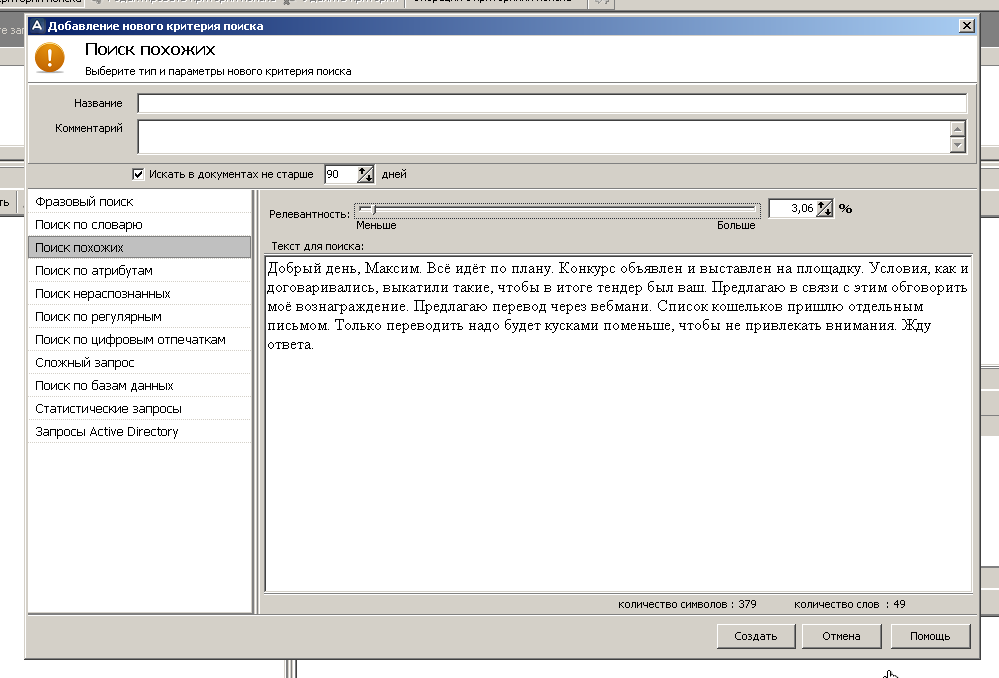
\includegraphics[width=\textwidth]{part3/1}
\end{figure}

\begin{figure}[H]
  \centering
  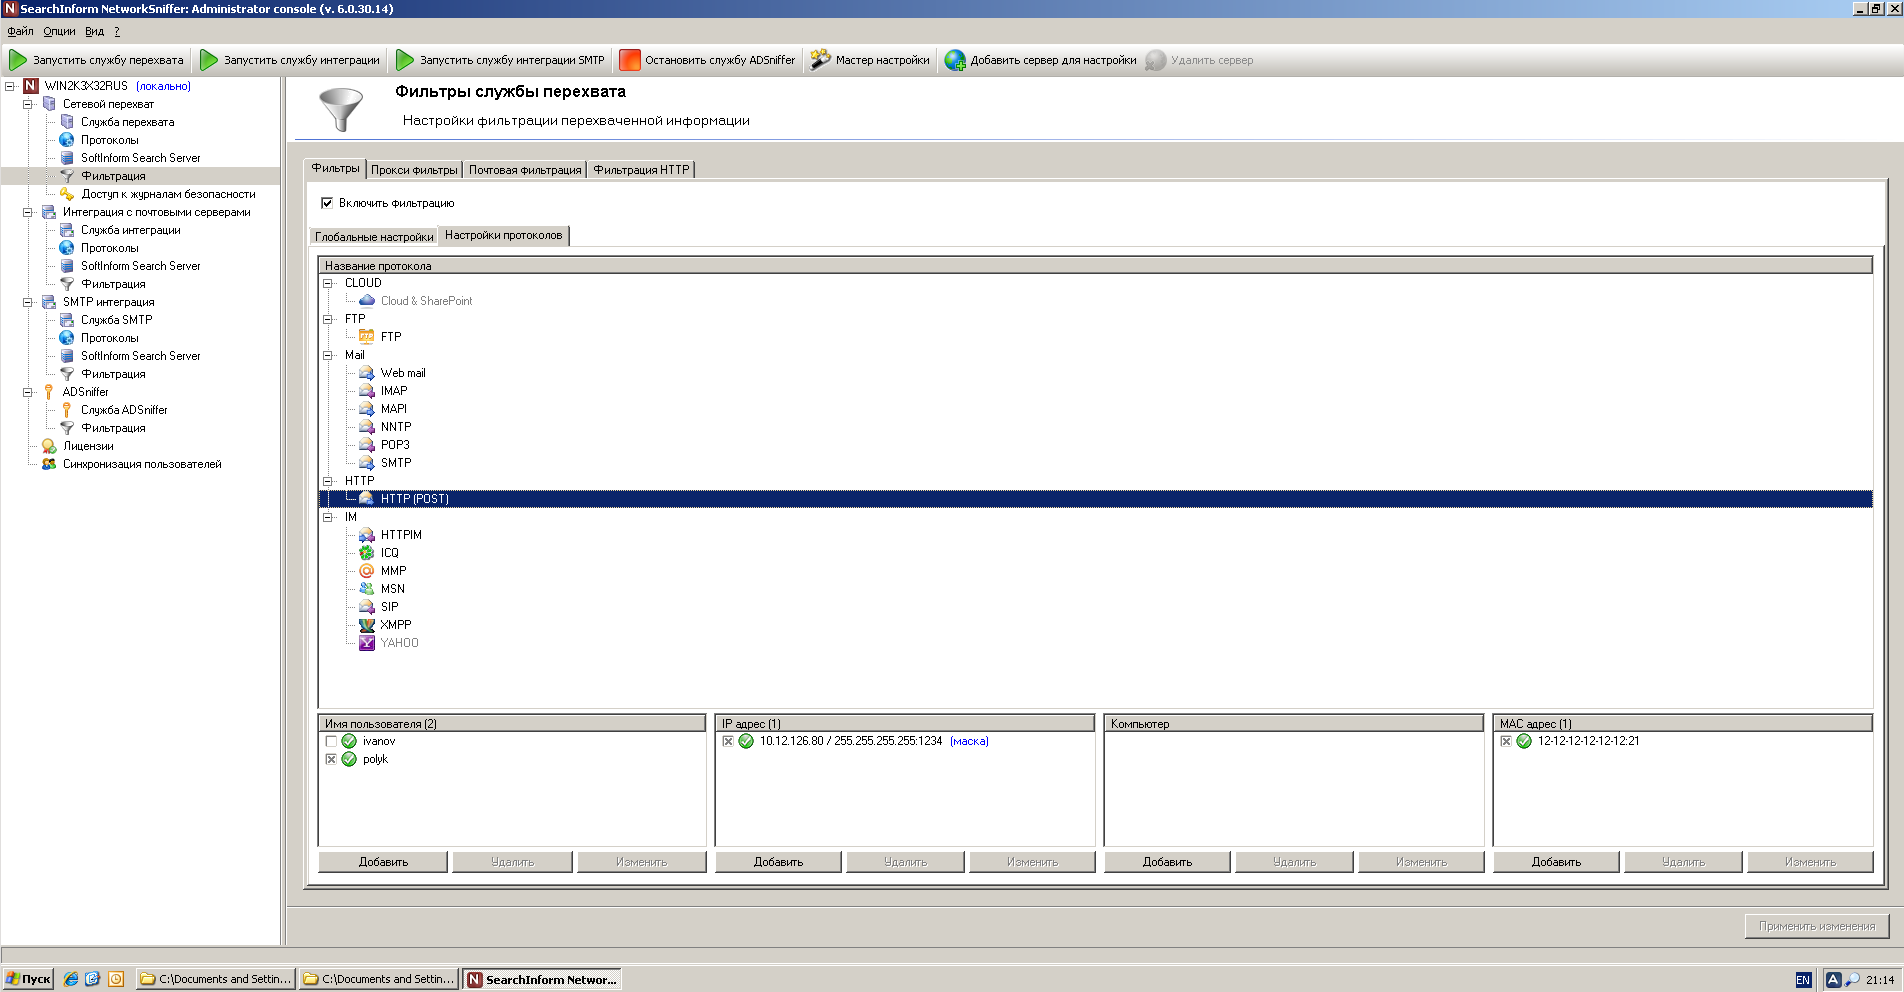
\includegraphics[width=\textwidth]{part3/2}
\end{figure}

\begin{figure}[H]
  \centering
  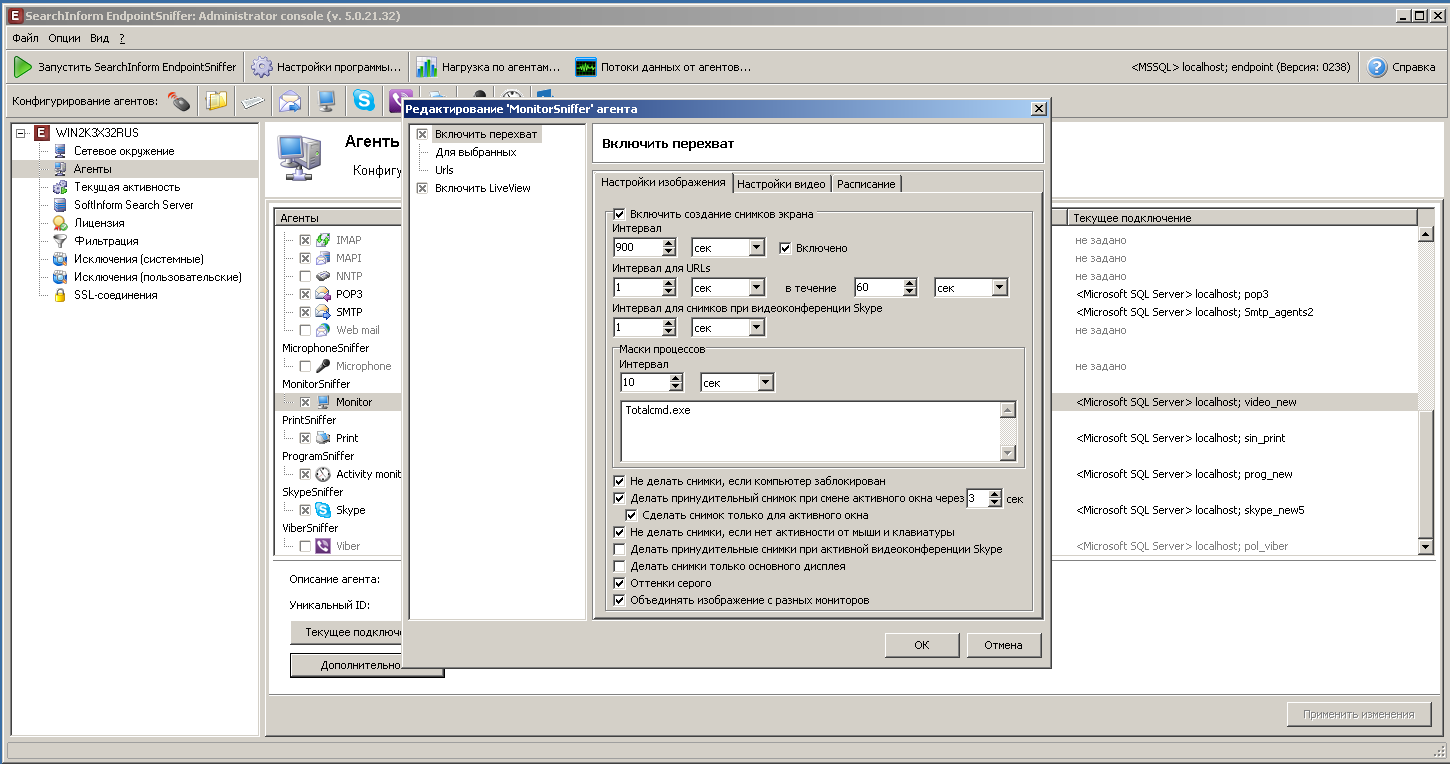
\includegraphics[width=\textwidth]{part3/3}
\end{figure}

\begin{figure}[H]
  \centering
  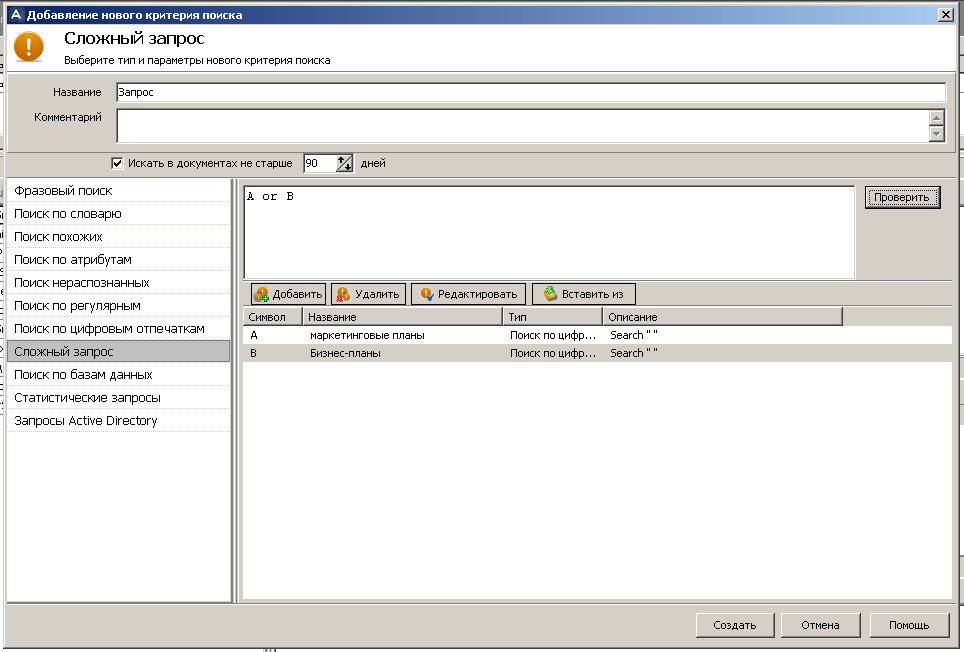
\includegraphics[width=\textwidth]{part3/4}
\end{figure}

\begin{figure}[H]
  \centering
  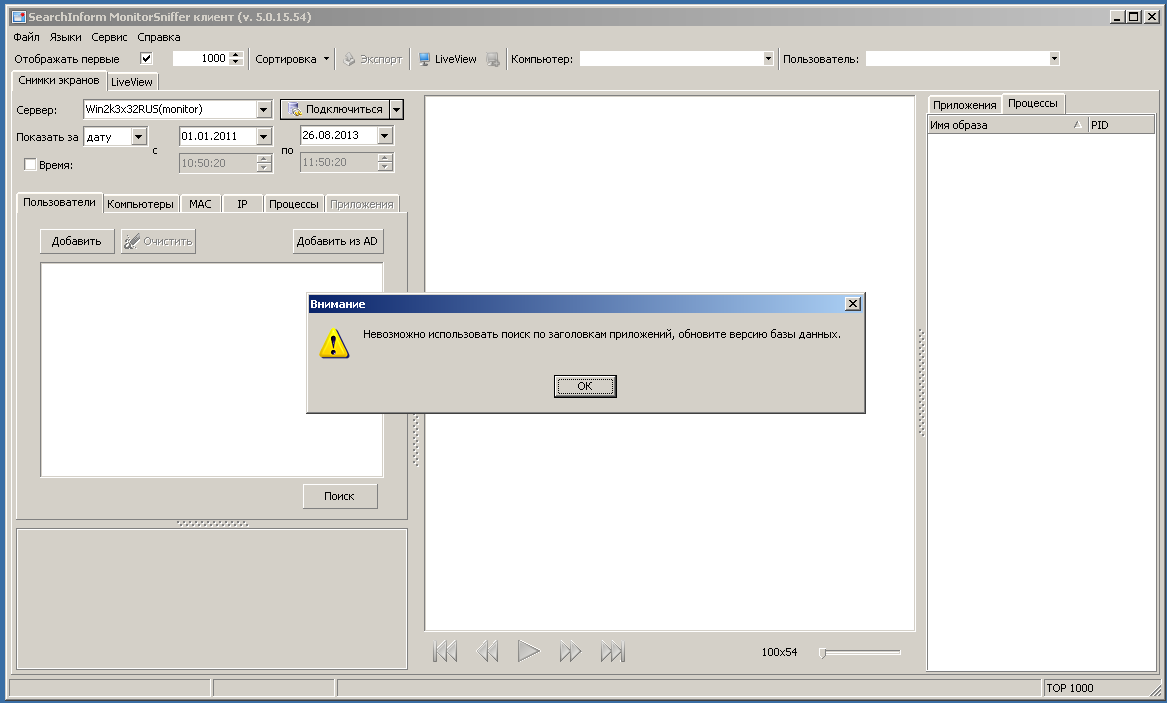
\includegraphics[width=\textwidth]{part3/5}
\end{figure}

К сожалению, в свежей версии образа не обновленная база данных.

\begin{itemize}
  \item Почему количество снимков экрана отфильтрованных по определенному
    IP-адресу может отличаться от количества снимков отфильтрованных по
    MAC-адресу, который соответствует определенному IP?

    Несколько машин могут использовать один IP адрес.

  \item Зачем, кроме фильтрации снимков экрана по именам пользователя нужна
    фильтрация по  IP  и MAC-адресам?

    Пользователь может пользоваться не только одной машиной.

  \item Почему на данном виртуальном компьютере при текущей конфигурации
    программного комплекса SearchInform нельзя реализовать оперативный контроль
    за экраном пользователя?

    Конфигурация не эмулирует только сервер с SearchInform.

  \item Какое назначение опции LiveView агента MonitorSniffer?

    Просмотр действий пользователя.
\end{itemize}
